% Created 2023-01-11 Wed 12:20
% Intended LaTeX compiler: pdflatex
\documentclass{report}
                              \usepackage[utf8]{inputenc}
\usepackage[T1]{fontenc}
\usepackage{RJournal}
\usepackage{amsmath,amssymb,array}
\usepackage{booktabs}
\sectionhead{Contributed research article}
\volume{XX}
\volnumber{ZZ}
\year{20YY}
\month{MM}
\usepackage{blindtext}
\usepackage{xcolor}
\usepackage{listings}
\usepackage{hyperref}
\hypersetup{colorlinks=true, linkcolor=blue, filecolor=magenta, urlcolor=cyan}
\usepackage{float}
\DeclareMathOperator*{\argmax}{argmax}
\DeclareMathOperator*{\argmin}{argmin}
\newcommand{\J}{\ensuremath{J}}
\newcommand{\1}{\ensuremath{\mathbf{1}}}
\newcommand{\h}{\ensuremath{\lambda}}
\newcommand{\indep}{\ensuremath{\perp\hspace*{-1.4ex}\perp}}
\newcommand{\T}{\ensuremath{\widetilde{T}}}
\newcommand{\X}{\ensuremath{{W}}}
\renewcommand{\t}{\ensuremath{\Tilde{t}}}
\newcommand{\ax}{\ensuremath{\mid a,\,{w}}}
\newcommand{\aX}{\ensuremath{\mid A = a,\,{W}}}
\newcommand{\AX}{\ensuremath{\mid A,\,{W}}}
\newcommand{\x}{\ensuremath{{w}}}
\newcommand{\trt}{\ensuremath{\pi^*}}
\newcommand{\tk}{\ensuremath{t_{k}}}
\newcommand{\lj}{\ensuremath{l}}
\newcommand{\jj}{\ensuremath{j}}
\newcommand{\tK}{\ensuremath{K}}
\newcommand{\tKi}{\ensuremath{k}}
\newcommand{\TK}{\ensuremath{\mathcal{T}}}
\newcommand{\g}{\ensuremath{\pi}}
\renewcommand{\L}{\ensuremath{W}}
\renewcommand{\l}{\ensuremath{w}}
\newcommand{\tDelta}{\ensuremath{\widetilde{\Delta}}}
\setcounter{secnumdepth}{5}

\lstset{
keywordstyle=\color{blue},
commentstyle=\color{red},stringstyle=\color[rgb]{0,.5,0},
literate={~}{$\sim$}{1},
basicstyle=\ttfamily\small,
columns=fullflexible,
breaklines=true,
breakatwhitespace=false,
numbers=left,
numberstyle=\ttfamily\tiny\color{gray},
stepnumber=1,
numbersep=10pt,
backgroundcolor=\color{white},
tabsize=4,
keepspaces=true,
showspaces=false,
showstringspaces=false,
xleftmargin=.23in,
frame=single,
basewidth={0.5em,0.4em},
}
\renewcommand*\familydefault{\sfdefault}
\itemsep2pt
\author{imbroglio}
\date{\today}
\title{}
\begin{document}

\title{concrete R Paper}
\subtitle{}
\author{by David Chen, Thomas Gerds, Helene Rytgaard, Maya L. Petersen, Mark van der Laan, ...}

\maketitle

\abstract{
Recently targeted maximum likelihood-based estimation (TMLE) has been used to develop estimators of cause-specific absolute risks for time-to-event outcomes measured in continuous time. The point treatment continuous-time survival TMLE method is implemented in the \CRANpkg{concrete} package for `R`. \CRANpkg{concrete} provides methods to estimate intervention and cause-specific absolute risks as well as contrastive parameters such as risk differences and risk ratios. The package allows the risks of multiple causes to be jointly targeted in the case of competing risks, at multiple time points and in the presence of right-censoring. In this paper we describe and illustrate the usage of the \CRANpkg{concrete} package.
}

\section{Introduction}
\label{intro}
\CRANpkg{concrete} is a statistical estimation package written to help researchers answer causal questions about time-to-event outcomes in continous time. When we analyze data and make predictions to guide future actions we are in essence asking causal questions, questions that can be made rigorous using the formal causal inference frameworks developed in recent decades (\cite{pearl_causal_2016}, \cite{holland_statistics_1986}). However, the transition from causal thinking to statistical estimation is not always straightforward, and so a cohesive causal inference workflow should follow a structured roadmap (\cite{petersen_causal_2014}) that begins with the causal model and causal estimands, moves through identification to a statistical model and estimands, and then finally performs estimation and provides inference. Detailed discussions of these first two stages can be found elsewhere but will only be briefly discussed in this manuscript, as \CRANpkg{concrete} is fundamentally a statistical estimation package, albeit one that is written with this causal inference workflow in mind.

\subsection{What is in this manuscript}
\label{sec:orgd280fdf}
We write for readers looking for a hands-on introduction to the one-step targeted maximum likelihood estimation (TMLE) method for continuous time survival analysis described in \cite{rytgaard_one-step_2021}, as well as for readers
wishing to use this TMLE for their own continuous time survival or competing risks analyses. In Section \ref{concepts} we briefly overview the one-step TMLE method as it is implemented in \CRANpkg{concrete}
and in Section \ref{UsingConcrete} we show how to use \CRANpkg{concrete} for a continuous-time competing risks analysis. For a full and rigorous treatment of the one-step TMLE for continuous-time survival and competing risks analyses, see \cite{rytgaard_one-step_2021} and \cite{rytgaard_continuous-time_2021}.

\subsection{What can concrete be used for}
\label{sec:orgea8f43d}
\CRANpkg{concrete} can be used for targeted estimation of estimands derived from cause-specific absolute risks (e.g. relative risks and risk differences) under static and dynamic binary treatments given at baseline. The currently implemented estimators are the one-step TMLE and a g-formula plug-in, and both can be applied to data involving baseline covariate confounding, right-censoring and competing risks.

\CRANpkg{concrete} cannot yet investigate stochastic interventions or interventions on continuous or multinomial treatments. Methods have not yet been implemented to account for paired or clustered data, time-dependent treatments (e.g. drop-in) or time-dependent confounding. Currently only Cox models can be used for initial estimation of conditional hazards; incorporation of estimators based on highly adaptive lasso (HAL) and penalized cox is planned for future package versions.

\CRANpkg{concrete} is not meant to be used for left trunctation (i.e. delayed entry) or interval censored data and it will not check identification assumptions. 

\subsection{How concrete relates to other peoples work}
\label{sec:org6590b21}
\CRANpkg{concrete} will be the first R package implementing TMLE for continuous-time survival. The \CRANpkg{ltmle} (\cite{schwab_ltmle_2020}), \CRANpkg{stremr} (\cite{sofrygin_stremr_2017}), and \CRANpkg{survtmle} (\cite{benkeser_survtmle_2019}) packages either natively or can be adapted to perform discrete-time TMLE for absolute risks of right-censored survival outcomes; \CRANpkg{ltmle} and \CRANpkg{stremr} use the method of iterated expectations while \CRANpkg{survtmle} can target the hazard-based survival formulation. Notably these packages all work in discrete time and would necessitate discretizing continuous-time data, a practice which can in cases introduce bias and decrease estimator efficiency. 

The \ctv{Causal Inference} CRAN Task View shows just \CRANpkg{riskregression} (\cite{gerds_riskregression_2022}) as expressly estimating treatment effect estimands in survival settings. \CRANpkg{riskregression} implements the g-formula plug-in, IPTW, and double-robust AIPTW estimators. The \ctv{Survival} CRAN Task View shows no packages to be implementing efficient semi-parametric estimators for survival estimands, while not yet available on CRAN are the packages \href{https://github.com/RobinDenz1/adjustedCurves}{adjustedCurves} (\cite{denz_comparison_2022}) and \href{https://github.com/tedwestling/CFsurvival}{CFsurvival} (\cite{westling_inference_2021}) which implement the AIPTW and a cross-fitted doubly-robust estimator respectively. 

\subsection{What concrete does}
\label{sec:orgfa68819}
\CRANpkg{concrete} implements the one-step TMLE developed in \cite{rytgaard_one-step_2021} to estimate cause and intervention specific absolute risks, with asymptotic inference derived from the variance of the efficient influence curve (EIC) (\cite{laan_unified_2003-1}). \CRANpkg{concrete} can also return risk differences and risk ratios computed from these absolute risks with inference derived using the delta method on the EICs of the constituent absolute risks.

Broadly speaking, this one-step TMLE procedure consists of two stages: 1) an initial estimation of nuisance parameters and 2) a targeted update of the initial estimators to solve the EIC of the target statistical estimand (\cite{laan_unified_2003-1}, \cite{kennedy_semiparametric_2016}).

As it is often impossible to know in advance which estimator is best suited for a particular estimation problem, the use of a cross-validated machine learning ensemble with oracle guarantees (Super Learner \cite{laan_super_2007}, \cite{polley_superlearner_2021}, \cite{laan_unified_2003}, \cite{vaart_oracle_2006}) is helpful for the initial estimation of nuisance parameters. A Super Learner with a robust candidate library and a suitable loss function gives users the best chance of achieving the necessary nuisance estimation convergence rates for TMLE to be consistent and efficient. Guidance on how to best specify Superlearner estimators are discussed further in \cite{phillips_practical_2022}. Whenever possible, Super Learner libraries should include the highly adaptive lasso (HAL) which achieves the needed convergence rate (\cite{laan_generally_2017,benkeser_highly_2016,rytgaard_continuous-time_2021}) for TMLE's asymptotic properties.

The subsequent targeted update is based in semi-parametric efficiency theory (\cite{laan_targeted_2011}, \cite{kennedy_semiparametric_2016}), specifically that a regular, asymptotically linear estimator of a statistical estimand is efficient if its influence function is equal to the target estimand's EIC. By updating initial estimators of nuisance parameters to solve the EIC, TMLE recovers asymptotically valid inference despite potentially using flexible algorithms without well understood limiting behaviour for initial estimation.

\subsection{concrete in a nutshell - PBC example}
\label{sec:orge88e587}
\lstset{language=r,label=pbc nutshell,caption= ,captionpos=b,numbers=none,otherkeywords={}, deletekeywords={}}
\begin{lstlisting}
# Prepare Data
library(concrete)
library(data.table)
library(tidyverse)
set.seed(12345)
data <- as.data.table(survival::pbc)
data <- data[!is.na(trt), ][, trt := trt - 1]
data <- data[, c("time", "status", "trt", "age", "sex", "albumin")]

# Specify Analysis
ConcreteArgs <- formatArguments(DataTable = data,
				EventTime = "time",
				EventType = "status",
				Treatment = "trt",
				Intervention = makeITT(),
				TargetTime = 90 * (6:30),
				TargetEvent = 1:2,
				MaxUpdateIter = 250)
# Compute
ConcreteEst <- doConcrete(ConcreteArgs)

# Return Output
ConcreteOut <- getOutput(ConcreteEst)
plot(ConcreteOut, Estimand = "RR", GComp = FALSE)
\end{lstlisting}

\begin{figure}[H]
\center
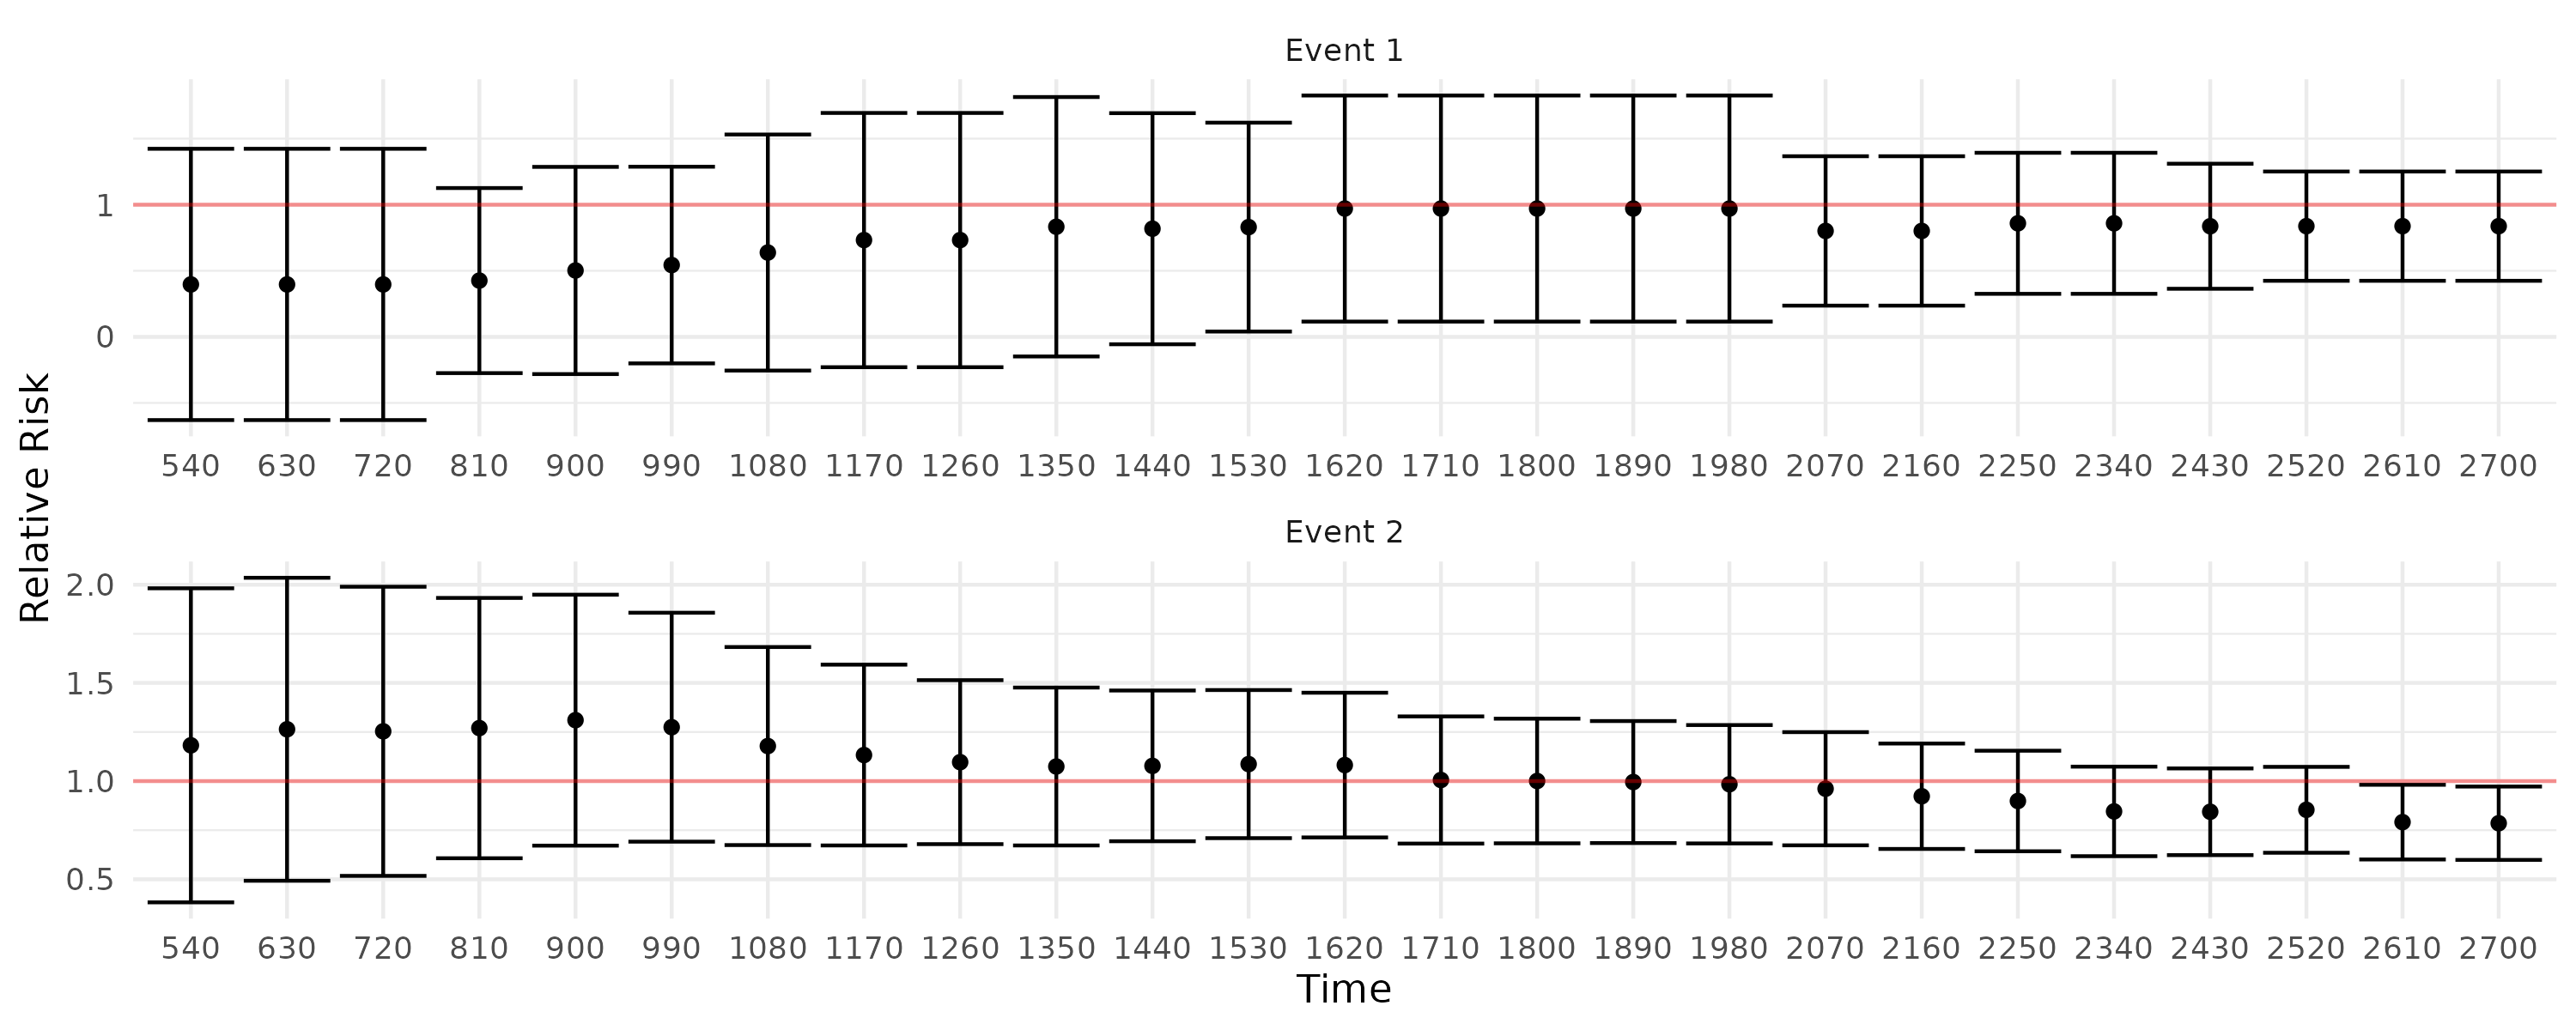
\includegraphics[width=\linewidth]{fig/RR.png}
\end{figure}

\section{Concepts}
\label{concepts}
\subsection{The Targeted Learning Roadmap}
\label{sec:org5a02990}
A basic targeted learning roadmap for analyzing continuous-time survival or competing risks consists of:
\begin{enumerate}
  \item Defining the causal model and specifying the causal estimand (e.g. causal risk difference at time $t$). Considerations include defining a time zero and a time horizon, specifying the event(s) of interest, identifying the intervention (i.e. treatment) variable and specifying the desired intervention(s).
  \item Stating the assumptions needed to define a statistical model with a statistical estimand that identifies the causal estimand. Considerations include identifying confounding variables and sources of right-censoring, establishing positivity for remaining uncensored and following desired interventions, and formalizing knowledge about the statistical model (e.g. dependency structure or functional structures such as proportional hazards)
  \item Estimation and inference. Considerations include pre-specification, estimator consistency and efficiency within a desired class, and both theoretical and practical robustness and usability.
\end{enumerate}

\subsection{The Causal Model: Counterfactuals, Interventions, and Causal Estimands}
\label{sec:org3401550}
With time-to-event data, the counterfactual outcome is the time until some event(s) occur to subjects if they hypothetically received an intervention. Let \(A\) be this intervention variable and let \(d\) be the intervention rule, i.e. the function that assigns values to \(A\). The simplest interventions are static rules to set \(A\) to some value \(a\), \(d = a\). A more flexible dynamic treatment rule might assign treatments based on subjects' baseline covariates, while stochastic treatment rules may even depend on the natural treatment assignment mechanism. Whatever the desired intervention, let \(d\) represent the intervention of interest and let \(\L\) represent a subject's baseline covariates. Then a counterfactual survival dataset with \(J\) competing events, an intervention \(d\) delivered at baseline time zero, and a time horizon of \(t_{max}\) takes the form:
\begin{equation}
 X = \left(\T^d,\, \Delta^d,\, \L \right) \quad,\quad T^d \in (0, t_{max}] \label{causaldata}
\end{equation}
\(\T^d \in \mathbb{R}^+\) is earliest occurence of any of the \(J\) events under intervention \(d\) and \(\Delta^d \in \{1, \dots, J\}\) shows which of the \(J\) events occured first under intervention \(d\).

Importantly, counterfactual data does not incorporate censoring; the counterfactual events are only those events that experimenters would allow to occur in their ideal hypothetical experiment. If the ideal experiment would track just the incidence of one event, then the causal problem is one of classic survival; if multiple events would be allowed to compete, then the causal problem is one with competing risks. 

Causal estimands can then be described as functions of this counterfactual data. For instance, to contrast the effects of interventions \(d^*\) and \(d^{**}\), we can write the causal event-\(j\) relative risk at time \(t\) as Eq. \eqref{causalrisk} and the causal difference in event-free survival at time \(t\) as Eq. \eqref{causalsurv}. 

\begin{equation}
P(T^{d^*}_j \leq t, \Delta^{d^*} = j) / P(T^{d^{**}}_j \leq t, \Delta^{d^{**}} = j) \label{causalrisk}
\end{equation}

\begin{equation}
P(T^{d^*}_j < t) - P(T^{d^{**}}_j < t) \label{causalsurv}
\end{equation}

Researchers may also be interested in these estimands at multiple timepoints, potentially up to the full risk curves over some time interval, and in the case of competing risks potentially for multiple event types as well.

\subsection{Observed Data, Identification, and Statistical Estimands}
\label{ObservedData}
Observed survival data with \(J\) competing events takes the form:
\begin{equation}
 O = \left(\T,\, \tDelta,\, A,\, \L \right) \label{obs-data}
\end{equation}
where \(\T \in (0, t_{max}]\) is the earlier of the first event time or the right-censoring time, \(\tDelta \in \{0, \dots, J\}\) indicates which event occurs (with 0 indicating right-censoring), \(A\) is the observed intervention and \(\L\) is the set of baseline covariates.

To link causal estimands such as Eq. \eqref{causalrisk} and \eqref{causalsurv} to statistical estimands, we need the following untestable identification assumptions to hold: consistency, positivity for treatments and remaining uncensored, no unmeasured confounding, and coarsening at random on the censoring process (details in Appendix \ref{identification}). Given these assumptions, the cause-\(j\) absolute risk at time \(t\) under intervention \(d\) is identified by the g-computation formula
\begin{align}
F^d_j(t) &= \mathbb{E}_{\mathcal{\L}} \left[ \mathbb{E}_{\g^d} \left[{\color{blue!50!green} F_j(t \ax)} \right] \right] \nonumber \\
&= \mathbb{E}_{\mathcal{\L}} \left[ \int_{\mathcal{A}} \,  \left[{\color{blue!50!green} \int_0^t \lambda_j(s \ax) \, S(s- \ax) \, ds }\right] \, \g^d (a \mid \l) \, da \right] \label{absrisk}
\end{align}
where
\(\lambda_j(t \ax) = \lim\limits_{h \to 0} \frac{1}{h} P(\T \leq t + h,\, \tDelta = j \mid \T \geq t,\, a,\, \x)\) is the cause-\(j\) conditional hazard,\\
\(S(t \ax) = \exp\left(-\int^{t}_{0} \sum\limits_{j=1}^{J} \lambda_j(s \ax) \, ds \right)\) is the conditional event-free survival, and \(\g^d(a \mid \l)\) is the treatment propensity implied by the intervention \(d\). With the identification result in Eq. \eqref{absrisk}, the causal absolute risk \eqref{causalrisk} and survival \eqref{causalsurv} estimands can then be identified by statistical estimands \eqref{obsrisk} and \eqref{obssurv}.
\begin{equation}
\mathbb{E}_{\mathcal{\L}} \left[ \mathbb{E}_{\g^*} \left[ F_j(t \ax) \right] \right] / \; \mathbb{E}_{\mathcal{\L}} \left[ \mathbb{E}_{\g^{**}} \left[ F_j(t \ax) \right] \right] \label{obsrisk}
\end{equation}
\begin{equation}
\left[1 - \sum_{j = 1}^{J} \, \mathbb{E}_{\mathcal{\L}} \left[ \mathbb{E}_{\g^*} \left[ F_j(t \ax) \right] \right] \right] - \left[1 - \sum_{j = 1}^{J} \, \mathbb{E}_{\mathcal{\L}} \left[ \mathbb{E}_{\g^{**}} \left[ F_j(t \ax) \right] \right] \right] \label{obssurv}
\end{equation}
It should be noted that even if the identification assumptions do not hold, these statistical estimands in Eq. \eqref{obsrisk} and \eqref{obssurv} may still have valuable interpretations as standardized risks isolating the importance of the "intervention" variable (\cite{laan_statistical_2006}).

\subsection{Estimation}
\label{estimation}
\CRANpkg{concrete} implements the one-step continuous time TMLE for estimands derived from cause-specific, intervention-specific absolute risks, which begins with estimating the treatment propensity \(\g\), the conditional hazard of censoring \(\lambda_c\) and the conditional hazard of each event \(\lambda_j \,:\; j = 1, \dots, J\). Super Learners are used to estimate these nuisance parameters, which involves specifying the cross-validation scheme, libraries of candidate algorithms, the cross-validation loss functions, and the Super Learner meta-learner.

\subsubsection{Cross-Validation}
\label{cv}
For a \(V\text{-fold}\) cross validation scheme, let \(Q_n = \{O_i\}_{i=1}^n\) be the observed \(n\) i.i.d observations of \(O \sim P_0\) and let \(B_n = \{1, ... , V\}^n\) be a random vector that assigns the \(n\) observations into \(V\) validation folds. For each \(v \in \{1, ..., V\}\) we then define a training set \(Q^\mathcal{T}_v = \{O_i : B_n(i) = v\}\) with the corresponding validation set \(Q^\mathcal{V}_v = \{O_i : B_n(i) \neq v\}\). For guidelines on selecting the number of folds and when stratification may be helpful, it may be helpful to consult \cite{phillips_practical_2022}. 

Libraries should be constructed from candidate algorithms that vary in flexibility and respect pre-existing knowledge about the data-generating mechanism. For instance, Cox models should incorporate domain knowledge about which covariates may be most predictive of event times and if \(n\) is much greater than the number of covariates then more flexible candidate Cox parameterizations along with flexible algorithms such as Highly Adaptive Lasso (HAL). If on the other hand the number of covariates is not much smaller \(n\), then fewer and less flexible candidate algorithms should be used, potentially either including penalization natively or being paired with covariate screening algorithms.

Super Learner candidates should be evaluated on a cross-validated loss function that is minimized by the true data-generating process and for maximal robustness a discrete selector that simply selects the best performing candidate should be used as the Super Learner metalearner.

\subsubsection{Initial Estimate of Treatment Propensity}
\label{trtps-est}
For estimating the treatment propensity, let \(\g_0(\cdot \mid \X)\) be the true conditional distribution of \(A\) given \(\X\), \(\mathcal{M}_{\g} = \left\{\Hat{\g} : Q_n \to \Hat{\g}(Q_n) \right\}\) be the candidate library of propensity score estimators, and \(L_\g\) be a loss function such that the risk \(\mathbb{E}_0\left[L_\g(\Hat{\g}, O)\right]\) is minimized when \(\Hat{\g} = \g_0\). The discrete Superlearner estimator is then the the candidate propensity estimator \(\Hat{\g} \in \mathcal{M}_{\g}\) that has minimal cross validated risk
\begin{equation}
\Hat{\g}^{SL} = \argmin_{\Hat{\g} \in \mathcal{M}_\g} \sum_{v = 1}^{V} P_{Q^\mathcal{V}_v} \; L_\g(\Hat{\g}(Q^\mathcal{T}_v), Q^\mathcal{V}_v) \label{propsl}
\end{equation}

\subsubsection{Initial Estimate of Conditional Hazards}
\label{haz-est}
For estimating the conditional hazards, let \(\lambda_{0,\,\delta} \,:\; \delta = 0, \dots, J\) be the true conditional hazards for censoring (\(\delta = 0\)) and events (\(\delta \in \{1, \dots, J\}\)). Let \(\mathcal{M}_\delta = \{\Hat{\lambda}_\delta : Q_n \to \mathbb{R}\}\) for \(\delta = 0, \dots, J\) be the libraries of candidate Cox hazard specifications for the censoring and cause-specific hazards and let \(L_\delta(\beta) = - \sum_{i=1}^{n} \left[\beta\,\L_i - \log\left[\sum_{h \in \mathcal{R}(\T_h)} \exp(\beta\,\L_h)\right]\right] \,\) be the negative log Cox partial-likelihood loss function. The discrete SuperLearner selector for each \(\delta\) chooses the candidate \(\Hat{\lambda}_\delta \in \mathcal{M}_\delta\) that has minimal cross validated risk 
\begin{equation}
\Hat{\lambda}_\delta^{SL} = \argmin_{\Hat{\lambda}_\delta \in \mathcal{M}_\delta} \sum_{v = 1}^{V} P_{Q^\mathcal{V}_v} \; L_\g(\Hat{\lambda}_\delta(Q^\mathcal{T}_v), Q^\mathcal{V}_v) \;:\; \delta = 0, \dots, J\label{hazsl}
\end{equation}

\subsubsection{Efficient Influence Curve}
\label{EIC}
The treatment propensity estimator Eq. \eqref{propsl} and conditional hazard estimators Eq. \eqref{hazsl} are used to estimate the nuisance parameters that make up the EICs of absolute-risk derived estimands like Eq. \eqref{obsrisk} and \eqref{obssurv}. Parameters that contrast multiple cause-specific absolute risks at multiple time points involve vector EICs comprised of the absolute risk EICs for each targeted event, each target time, and each intervention. For the event \(\jj\), time \(t\), and intervention propensity \(\trt\) absolute risk (\(\Psi_{\trt, \jj, t}(P_0) = F_\jj^{\trt}(t)\)), the corresponding vector EIC element is:
\begin{align}
    D^*_{\trt, \jj, t}(\lambda, \g, S_c)(O) = \sum_{\lj = 1}^{J} \int \; &h_{\trt,\, \jj,\, \lj,\, t, s}(\lambda, \g, S_c)(O) \, \left(N_{\lj}(ds) - \1(\T \geq s) \, \lambda_\lj(s \AX)\right) \label{eic} \\
    &{\color{blue!60!black}+ \sum_{a\,\in\,\mathcal{A}} F_\jj(t \mid A = a, \X)\,\trt(a \mid \X) - \Psi_{\trt, \jj, t}(P_0)}  \nonumber 
\end{align}
where \(N_l(s) = \1\left\{\T \leq s, \tDelta = l\right\}\) are the cause-specific counting processes and \(h_{\trt,\, \jj,\, \lj,\, t,\, s}(\lambda, \g, S_c)(O)\) is the TMLE "clever covariate" with the form
\begin{align}
    h_{\trt,\, \jj,\, \lj,\, t,\, s}&(\lambda, \g, S_c)(O) = \frac{{\color{blue}\trt(A \mid \X)\,} \1(s \leq t)}{{\color{green!70!black}\g(A \mid \X) \;S_c(s\text{-} \AX)}} \, \bigg(\1(\Delta = \jj) - \frac{{\color{red}F_\jj(t \AX)} - {\color{red} F_\jj(s \AX)}}{{\color{red} S(s \AX)}}\bigg) \label{clevcov}
\end{align}
where \(F_j(t \ax)\) is the conditional cause-\(j\) absolute risk, \(S_c(t \AX)\) is the conditional censoring survival, \(S(t \AX)\) is the conditional event-free survival, and \(N_j(t) = \1\{\T \leq t, \, \Delta = l\}\) is the event-\(j\) counting process. The treatment propensity \(\g\) and the conditional event and censoring hazard functions ( \(\lambda_c,\, \lambda_j \;:\;  j = 1, \dots, J\)) are directly estimated with Eq. \eqref{propsl} and \eqref{hazsl} while the conditional absolute risks and survivals are computed from the hazard estimates as described in Section \ref{ObservedData}. The clever covariate is a function of the {\color{blue}intervention propensity}, {\color{green!70!black}observed conditional distributions} which are not changed by TMLE targeting, and lastly the {\color{red}outcome-related conditional distributions} which are updated by targeting.

The one-step continuous-time survival TMLE updates the cause-specific hazards along the universally least favorable submodel in the following manner:
\begin{equation}
\lambda_{j, \epsilon}(t) = \lambda_{j}(t) \, \exp\left(\int_{0}^{\epsilon}\frac{\left<\mathbb{P}_n \tilde{D}^*( \lambda_{x}, \g,  S_c)(O),\; h_{j, s}( \lambda_{x}, \g,  S_c)(O) \right>_{\Sigma}}{|| \tilde{D}^*( \lambda_{x}, \g, S_c)(O)||_{\Sigma}} \; dx \right) \label{onestep}
\end{equation}
where
\begin{align*}
\left<x , y \right>&_{\Sigma} = x^\top \Sigma^{\text{ -}1} y \hspace{.5cm}, \hspace{.5cm} ||x||_{\Sigma} = \sqrt{x^\top \Sigma^{\text{ -}1} x}
\intertext{\(\tilde{D}^*\) is the vector of efficient influence functions}
\tilde{D}^{*}(\lambda, \g, S_c)(O) &= \left(D^*_{\trt, \jj, \tk}(\lambda, \g, S_c)(O) : \trt \in \mathcal{A}, \jj \in \mathcal{J}, \tk \in \TK)\right)
\intertext{and \(h_{j, s}\) is the vector of clever covariates}
h_{j, s}(\lambda, \g, S_c)(O) &= \left(h_{\trt, \jj, \lj, \tk, s}(\lambda, \g, S_c)(O) : \trt \in \mathcal{A}, \jj \in \mathcal{J}, \tk \in \TK)\right)
\end{align*}
In practice this integral is approximated by recursively summing along a series of locally least favorable models and ends when 

\begin{equation}
\mathbb{P}_n D^*(\lambda_{\epsilon}, \g, S_c)(O) \leq \frac{\sqrt{\mathbb{P}_n \;D^*( \lambda_{\epsilon}, \g, S_c)(O)^2}}{\sqrt{n} \, \log(n)} \label{one-step-stop}
\end{equation}

\subsubsection{Variance Estimation}
\label{sec:org267b245}

\CRANpkg{concrete} estimates the variance of targeted risks by dividing the corresponding EIC's variance by the sample size, \(\frac{\mathbb{P}_n \;D^*( \lambda_{\epsilon}, \g, S_c)(O)^2}{n}\), which is a consistent estimator of the asymptotic variance of asymptotically linear estimators. In the presence of significant positivity violations (which may be seen as propensity scores close to 0), this EIC-derived variance estimator will be anti-conservative and variance estimation by bootstrap may be more reliable. However, bias resulting from positivity violations cannot be remedied in this way, and so other methods of addressing positivity violations (\cite{petersen_diagnosing_2012}) is recommended instead.

\section{Usage}
\label{UsingConcrete}
\CRANpkg{concrete} was written for causal analyses of time-to-event data, though it can also be used for purely statistical estimation problems. There are 3 main user-facing functions in \CRANpkg{concrete}: \code{formatArguments()}, \code{doConcrete}, and \code{getOutput}. Specification of the estimation problem is done through input into \code{formatArguments()}, which checks the estimation specification and return errors, warnings, and messages as necessary. The output of \code{formatArguments()} is a \code{"ConcreteArgs"} object which is then passed into \code{doConcrete()} to perform the specified continuous-time one-step survival TMLE. The output of \code{doConcrete()} is a \code{"ConcreteEst"} object which can be passed into getOutput to print, summarize, and plot cause-specific absolute risk derived estimands such as risk differences and relative risks. 

\subsection{formatArguments()}
\label{formatArguments}
Most inputs into \code{formatArguments()} are involved in specifying one of three tasks: specifying the observed data structure, the target estimand, or the TMLE update procedure. \code{formatArguments} sanity checks its arguments, i.e. the specified analysis, and returns an object of class \code{"ConcreteArgs"} with elements that can and sometimes should be modified by the user before passing the \code{"ConcreteArgs"} object back through \code{formatArguments} to be re-checked. This process can be repeated as necessary until the full estimation problem is adequately specified.

\subsubsection{Data}
\label{ObservedDataConcrete}
\CRANpkg{concrete} requires data to be in the general form described in Eq. \eqref{obs-data}, with the observed time to first event (censoring or otherwise) \(\T\), the indicator of which event occured (\(\Delta\), with \(\Delta = 0\) indicating right-censoring), the intervention variable \(A\), and a collection of baseline covariates \(\L\). This data must not include missing values; imputation of missing covariates should be done prior to passing data into \CRANpkg{concrete} while data with missing treatment or outcome values (other than right-censoring) is not supported by \CRANpkg{concrete}. Uniquely identifying subject IDs can be passed into \code{formatArguments()} through the \code{ID=} argument, though functionality for using subject IDs for analyzing clustered or longitudinal data has not yet been implemented.

Using the PBC dataset as our example, \(\T\) is the column \code{"time"}, \(\Delta\) is the column \code{"status"}, \(A\) is the column \code{"trt"}, and \(\L\) consists of all the columns containing patient information observed at baseline.  This data is passed into \CRANpkg{concrete} as the following:
\lstset{language=r,label=pbc formatargs silent,caption= ,captionpos=b,numbers=none,otherkeywords={}, deletekeywords={}}
\begin{lstlisting}
library(concrete)
library(data.table)
set.seed(0)
obs <- as.data.table(survival::pbc)
obs <- obs[,  c("time", "status", "trt", "id", "age", "albumin", "sex")]
obs <- obs[!is.na(trt), ]
ConcreteArgs <- formatArguments(DataTable = obs, EventTime = "time",
				EventType = "status", Treatment = "trt",
				ID = "id", Intervention = 0:1)
\end{lstlisting}

\subsubsection{Target Estimand}
\label{Estimand}
\CRANpkg{concrete} implements a continuous-time one-step TMLE targeting absolute risk derived estimands indexed by  interventions, target events, and target times.  

\paragraph{Intervention}
\label{TreatmentRegime}
For a binary \(A\) and static interventions \(d\) setting all observations to \(A=0\) or \(A=1\), then the intervention can specified \code{formatArguments(Intervention = c(0, 1)}.
\lstset{language=r,label= ,caption= ,captionpos=b,numbers=none,otherkeywords={}, deletekeywords={}}
\begin{lstlisting}
ConcreteArgs <- formatArguments(DataTable = obs, EventTime = "time",
				EventType = "status", Treatment = "trt",
				ID = "id", Intervention = 0:1)
\end{lstlisting}

More complex dynamic interventions are passed into \code{formatArguments(Intervention =)} as a list containing a pair of functions: an "intervention" function which outputs desired treatment \textbf{\textbf{assignments}} and a "g.star" function which outputs desired treatment \textbf{\textbf{probabilities}}. These functions can take treatment and covariates as arguments and must produce either treatment assignments or treatment probabilities respectively, each with the same dimensions as the observed treatment. The function \code{makeITT()} creates list of functions corresponding to binary static interventions, which can be used as a template for more complex interventions.

\paragraph{Target Events}
\label{TargetEvent}
The \code{TargetEvent = } argument specifies the event types of interest. For \CRANpkg{concrete} event types must be integer valued, with 0 by default reserved for censoring. If no input is supplied and the default \code{TargetEvent = NULL} is used, then all observed non-zero event types will be targeted. If input is supplied for \code{TargetEvent = }, then all other observed event types will be treated as right-censoring.

In the \code{pbc} dataset, there are 3 event values encoded by the \code{status} column: 0 for censored, 1 for transplant, and 2 for death. To analyze \code{pbc} with transplants treated as right-censoring, \code{TargetEvent} should be set to 2,
\lstset{language=r,label= ,caption= ,captionpos=b,numbers=none,otherkeywords={}, deletekeywords={}}
\begin{lstlisting}
ConcreteArgs <- formatArguments(DataTable = obs, EventTime = "time",
				EventType = "status", Treatment = "trt",
				ID = "id", Intervention = 0:1,
				TargetEvent = 2)
\end{lstlisting}
whereas for a competing risks analysis one could either leave \code{TargetEvent = NULL} or specify \code{TargetEvent = 1:2}
\lstset{language=r,label= ,caption= ,captionpos=b,numbers=none,otherkeywords={}, deletekeywords={}}
\begin{lstlisting}
ConcreteArgs <- formatArguments(DataTable = obs, EventTime = "time",
				EventType = "status", Treatment = "trt",
				ID = "id", Intervention = 0:1,
				TargetEvent = 1:2)
\end{lstlisting}

\paragraph{Target Time}
\label{TargetTime}
The \code{TargetTime=} argument specifies the time(s) at which estimates of the cause-specific absolute risks or event-free survival are desired. Target times should be restricted to the time range in which target events are observed and \code{formatArguments()} will return an error if target time is after the last observed failure event time. If no \code{TargetTime} is provided, then \CRANpkg{concrete} will target the last observed event time, though this is likely to result in a highly variable estimate if prior censoring is substantial. 

The \code{TargetTime=} argument can either be a single number or a vector, as one-step TMLE can target cause-specific risks at multiple times simultaneously. For estimands involving full curves, \code{TargetTime=} should be set to a fine grid covering the desired interval.

\lstset{language=r,label= ,caption= ,captionpos=b,numbers=none,otherkeywords={}, deletekeywords={}}
\begin{lstlisting}
ConcreteArgs <- formatArguments(DataTable = obs, EventTime = "time",
				EventType = "status", Treatment = "trt", ID = "id", 
				Intervention = 0:1, TargetEvent = 1:2, TargetTime = 90 * (16:24))
\end{lstlisting}


\subsubsection{Estimator Specification}
\label{EstimationSpec}
The \code{formatArguments()} arguments involved in estimation are the cross-validation setup \code{CVArg}, the Superlearner candidate libraries \code{Model}, the software backends \code{PropScoreBackend} and \code{HazEstBackend}, and the practical TMLE implementation choices \code{MaxUpdateIter}, \code{OneStepEps}, and \code{MinNuisance}. It should be noted here that \code{Model} is used here to conform with common usage in statistical software, rather than to refer to statistical or causal models. 

\paragraph{Cross-Validation}
\label{CV}
\CRANpkg{concrete} uses \CRANpkg{origami} to specify cross-validation folds, specifically the function
\code{origami::make\_folds()}. If no input is provided to the \code{formatArguments(CVArg= )} argument, concrete will implement a simple 10-fold cross-validation scheme.

\lstset{language=r,label= ,caption= ,captionpos=b,numbers=none,otherkeywords={}, deletekeywords={}}
\begin{lstlisting}
CVArgs <- list(n = nrow(obs), V = 10L, fold_fun = folds_vfold, cluster_ids = NULL, strata_ids = NULL)

ConcreteArgs <- formatArguments(DataTable = obs, EventTime = "time", EventType = "status", 
				Treatment = "trt", ID = "id", 
				Intervention = 0:1, TargetEvent = 1:2, TargetTime = 90 * (16:24), 
				CVArg = CVArgs)
\end{lstlisting}

\paragraph{Estimating Nuisance Parameters}
\label{NuisanceEstimation}
\CRANpkg{concrete} accepts estimator specifications for estimating nuisance parameters through the argument \code{formatArguments(Model= )}. Inputs into the \code{Model=} argument must be named lists with one entry for the intervention variable, and for each of the event type including censoring. The list element corresponding to intervention must be named after the variable and the list elements corresponding to each event type must be named for the numeric value of the event type ("0" for censoring). If no input is provided for the \code{Model=} argument, \code{formatArguments()} will return a correctly formatted list, \code{.[["Model"]]}, containing default estimator specifications for each nuisance parameter, which can be then edited by the user.

\lstset{language=r,label= ,caption= ,captionpos=b,numbers=none,otherkeywords={}, deletekeywords={}}
\begin{lstlisting}
ConcreteArgs <- formatArguments(DataTable = obs, EventTime = "time", EventType = "status", 
				Treatment = "trt", ID = "id", 
				Intervention = 0:1, TargetEvent = 1:2, TargetTime = 90 * (16:24), 
				CVArg = NULL, Model = NULL)
str(ConcreteArgs[["Model"]], give.attr = FALSE)
\end{lstlisting}

\paragraph{Propensity Score}
\label{PropScore}
In \CRANpkg{concrete}, propensity scores are by default estimated using the \CRANpkg{SuperLearner}
package \code{formatArguments(PropScoreBackend = "Superlearner")} with candidate algorithms \code{c("xgboost", "glmnet")} implemented by packages \CRANpkg{xgboost} and \CRANpkg{glmnet}. Alternatively the \CRANpkg{sl3} package can be used by specifying \code{formatArguments(PropScoreBackend = "sl3")}.

\paragraph{Event and Censoring Hazards}
\label{HazardEstimation}
For estimating the necessary conditional hazards, \CRANpkg{concrete} currently relies on a discrete Superlearner consisting of a library of Cox models implemented by \code{survival::coxph()} evaluated on cross-validated pseuo-likelihood loss. Support for estimation of hazards using Poisson-HAL or other methods may be added in the future, but currently the \code{HazEstBackend} argument must be "coxph". The default Cox specifications are a treatment-only model and a main-terms model with treatment and all covariates.  

\lstset{language=r,label= ,caption= ,captionpos=b,numbers=none,otherkeywords={}, deletekeywords={}}
\begin{lstlisting}
DefaultHazardModels <- list("model1" = "~ trt", 
			    "model2" = "~ .")
\end{lstlisting}

\paragraph{One-step TMLE Specification}
\label{tmle-specification}
As detailed by Eq. \eqref{onestep} and \eqref{one-step-stop}, the one-step TMLE update step involves recursively updating cause-specific hazards, summing along small steps \(\epsilon_i\). The value of \(\epsilon\) is provided by the user as input into the argument \code{formatArguments(OneStepEps= )}; its default value is 0.1 and user-provided values must be between 0 and 1. The value of \code{OneStepEps} is meant to be heuristically small as the sum in Equation \eqref{onestep} approximates an integral; therefore \code{OneStepEps} is halved whenever an update step would increase the norm of the efficient influence function.

The \code{formatArguments(MaxUpdateIter= )} argument is provided to provide a definite stop to the recursive TMLE update. This argument takes positive integers and is set to a default of 100. More updates may be needed when support for targeted estimands in the data is low and when targeting estimands with many components.

The argument \code{formatArguments(MinNuisance= )} can be used to specify a lower bound for the product of the propensity score and lagged survival probablity for remaining uncensored; this term is present in the denominator of the efficient influence function and enforcing a lower bound decreases estimator variance at the cost of introducing bias. 

\lstset{language=r,label= ,caption= ,captionpos=b,numbers=none,otherkeywords={}, deletekeywords={}}
\begin{lstlisting}
ConcreteArgs <- formatArguments(DataTable = obs, EventTime = "time", EventType = "status", 
				Treatment = "trt", ID = "id", 
				Intervention = 0:1, TargetEvent = 1:2, TargetTime = 90 * (16:24), 
				CVArg = NULL, Model = NULL, 
				PropScoreBackend = "SuperLearner", HazEstBackend = "coxph", 
				MaxUpdateIter = 100, OneStepEps = 0.1, MinNuisance = 0.05)
\end{lstlisting}


\paragraph{ConcreteArgs object}
\label{concreteargs}
\code{formatArguments()} returns a list object of class \code{"ConcreteArgs"}. This object can be modified by the user and then passed back through \code{formatArguments()} in lieu of supplying new inputs directly into \code{formatArguments()}.

\lstset{language=r,label= ,caption= ,captionpos=b,numbers=none,otherkeywords={}, deletekeywords={}}
\begin{lstlisting}
ConcreteArgs <- formatArguments(DataTable = obs, EventTime = "time", EventType = "status", 
				Treatment = "trt", ID = "id", 
				Intervention = 0:1, TargetEvent = 1:2, TargetTime = 90 * (16:24), 
				CVArg = NULL, Model = ConcreteArgs[["Model"]], 
				PropScoreBackend = "SuperLearner", HazEstBackend = "coxph", 
				MaxUpdateIter = 100, OneStepEps = 1, MinNuisance = 0.05)

ConcreteArgs <- formatArguments(ConcreteArgs)
\end{lstlisting}

\subsection{doConcrete()}
\label{doConcrete}
Once \code{formatArguments()} runs satisfactorily, the resulting object of class \code{"ConcreteArgs"} can be passed into the \code{doConcrete()} function. \code{doConcrete()} will then perform the specified TMLE algorithm and output an object of class \code{"ConcreteEst"} which will contain contains TMLE point estimates and influence curves for the cause-specific absolute risks for each targeted event at each targeted time. If \code{formatArguments(GComp=TRUE)}, then the \code{"ConcreteEst"} object will also contain the result of using the Superlearner predictions as a plug-in g-formula estimate of the targeted risks. 

\lstset{language=r,label= ,caption= ,captionpos=b,numbers=none,otherkeywords={}, deletekeywords={}}
\begin{lstlisting}
ConcreteEst <- doConcrete(ConcreteArgs)
\end{lstlisting}

Detailed explanations of the one-step TMLE for continuous-time absolute risk derived estimands can be found in \cite{rytgaard_one-step_2021} and \cite{rytgaard_continuous-time_2021}. This manuscript briefly reviews this estimation procedure in Section \ref{estimation} and details how a TMLE is specified in \CRANpkg{concrete} in Section \ref{EstimationSpec}, subsections \ref{CV} through \ref{tmle-specification}. Here we will name the specific functions called in \code{doConcrete()} which perform each of the steps of the one-step continuous-time survival TMLE procedure.

The cross-validation specification (Section \ref{CV}) is checked and evaluated in \code{formatArguments()}, returning fold assignments as \code{.[["CVFolds"]]} of the \code{"ConcreteArgs"} object.

The initial estimation of nuisance parameters (Section \ref{NuisanceEstimation}) is performed by the function \code{getInitialEstimate()}; \code{getPropScore()} estimates propensity scores (Section \ref{PropScore}) and \code{getHazEstimate()} estimates the conditional hazards (Section \ref{HazardEstimation}).

The one-step TMLE update procedure (Sections \ref{estimation} and \ref{tmle-specification}, Equations \eqref{eic}, \eqref{clevcov}, \eqref{onestep}, and \eqref{one-step-stop}) is performed by \code{doTmleUpdate()} with \code{getEIC()} computing the efficient influence curves \eqref{eic}.

\subsection{getOutput()}
\label{getoutput}
\code{getOutput()} takes as an argument the \code{"ConcreteEst"} object returned by \code{doConcrete()} and returns tables and produces plots of the cause-specific risks, risk differences, and/or relative risks. By default \code{getOutput()} returns a data.table with point estimates and pointwise standard errors for cause-specific absolute risks, risk differences, and risk ratios. Risk difference and ratios are by default computed by subtracting or dividing the second listed intervention from the first. Below we show a subset of the relative risk estimates produced by the "nutshell" estimation specification for the pbc dataset. 

\lstset{language=r,label= ,caption= ,captionpos=b,numbers=none,otherkeywords={}, deletekeywords={}}
\begin{lstlisting}
getOutput(ConcreteEst, "RR", GComp = FALSE)[Time < 800 | Time > 2500, ]
\end{lstlisting}

\begin{figure}[H]
\centering
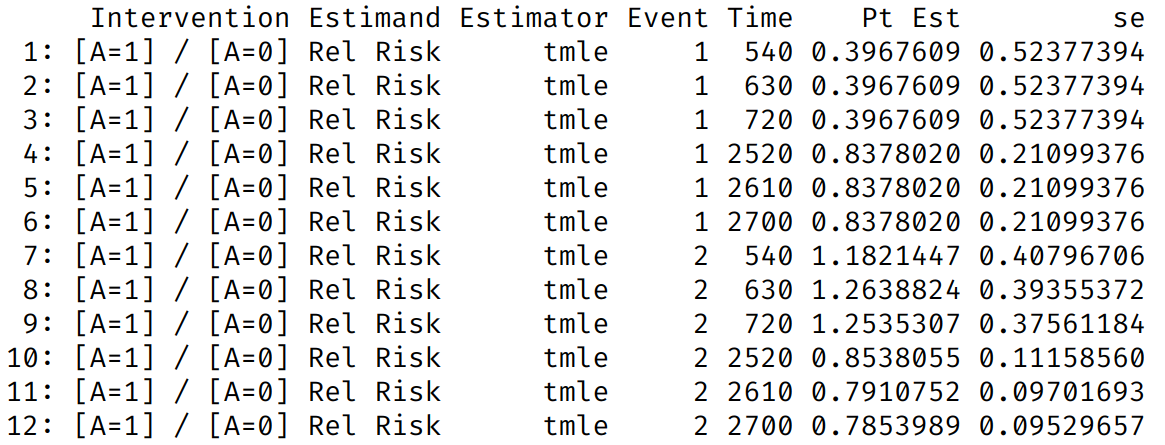
\includegraphics[width=.9\linewidth]{fig/rr-tbl.png}
\end{figure}

From this small sample risk ratios we can see that the treatment decreases the incidence of transplant (event 1) and leads to an increased incidence of death (event 2) earlier on followed by a decreased risk of death. We also see that these treatment effect estimates do not reach a 95\% level of significance. The full table is not shown here because it would take too much space, as can often be the case when estimands involve many time points. Instead results may be more easily interpreted when plotted, as we do below with the treated and control cause-specific risks for transplant and death.

\begin{figure}[H]
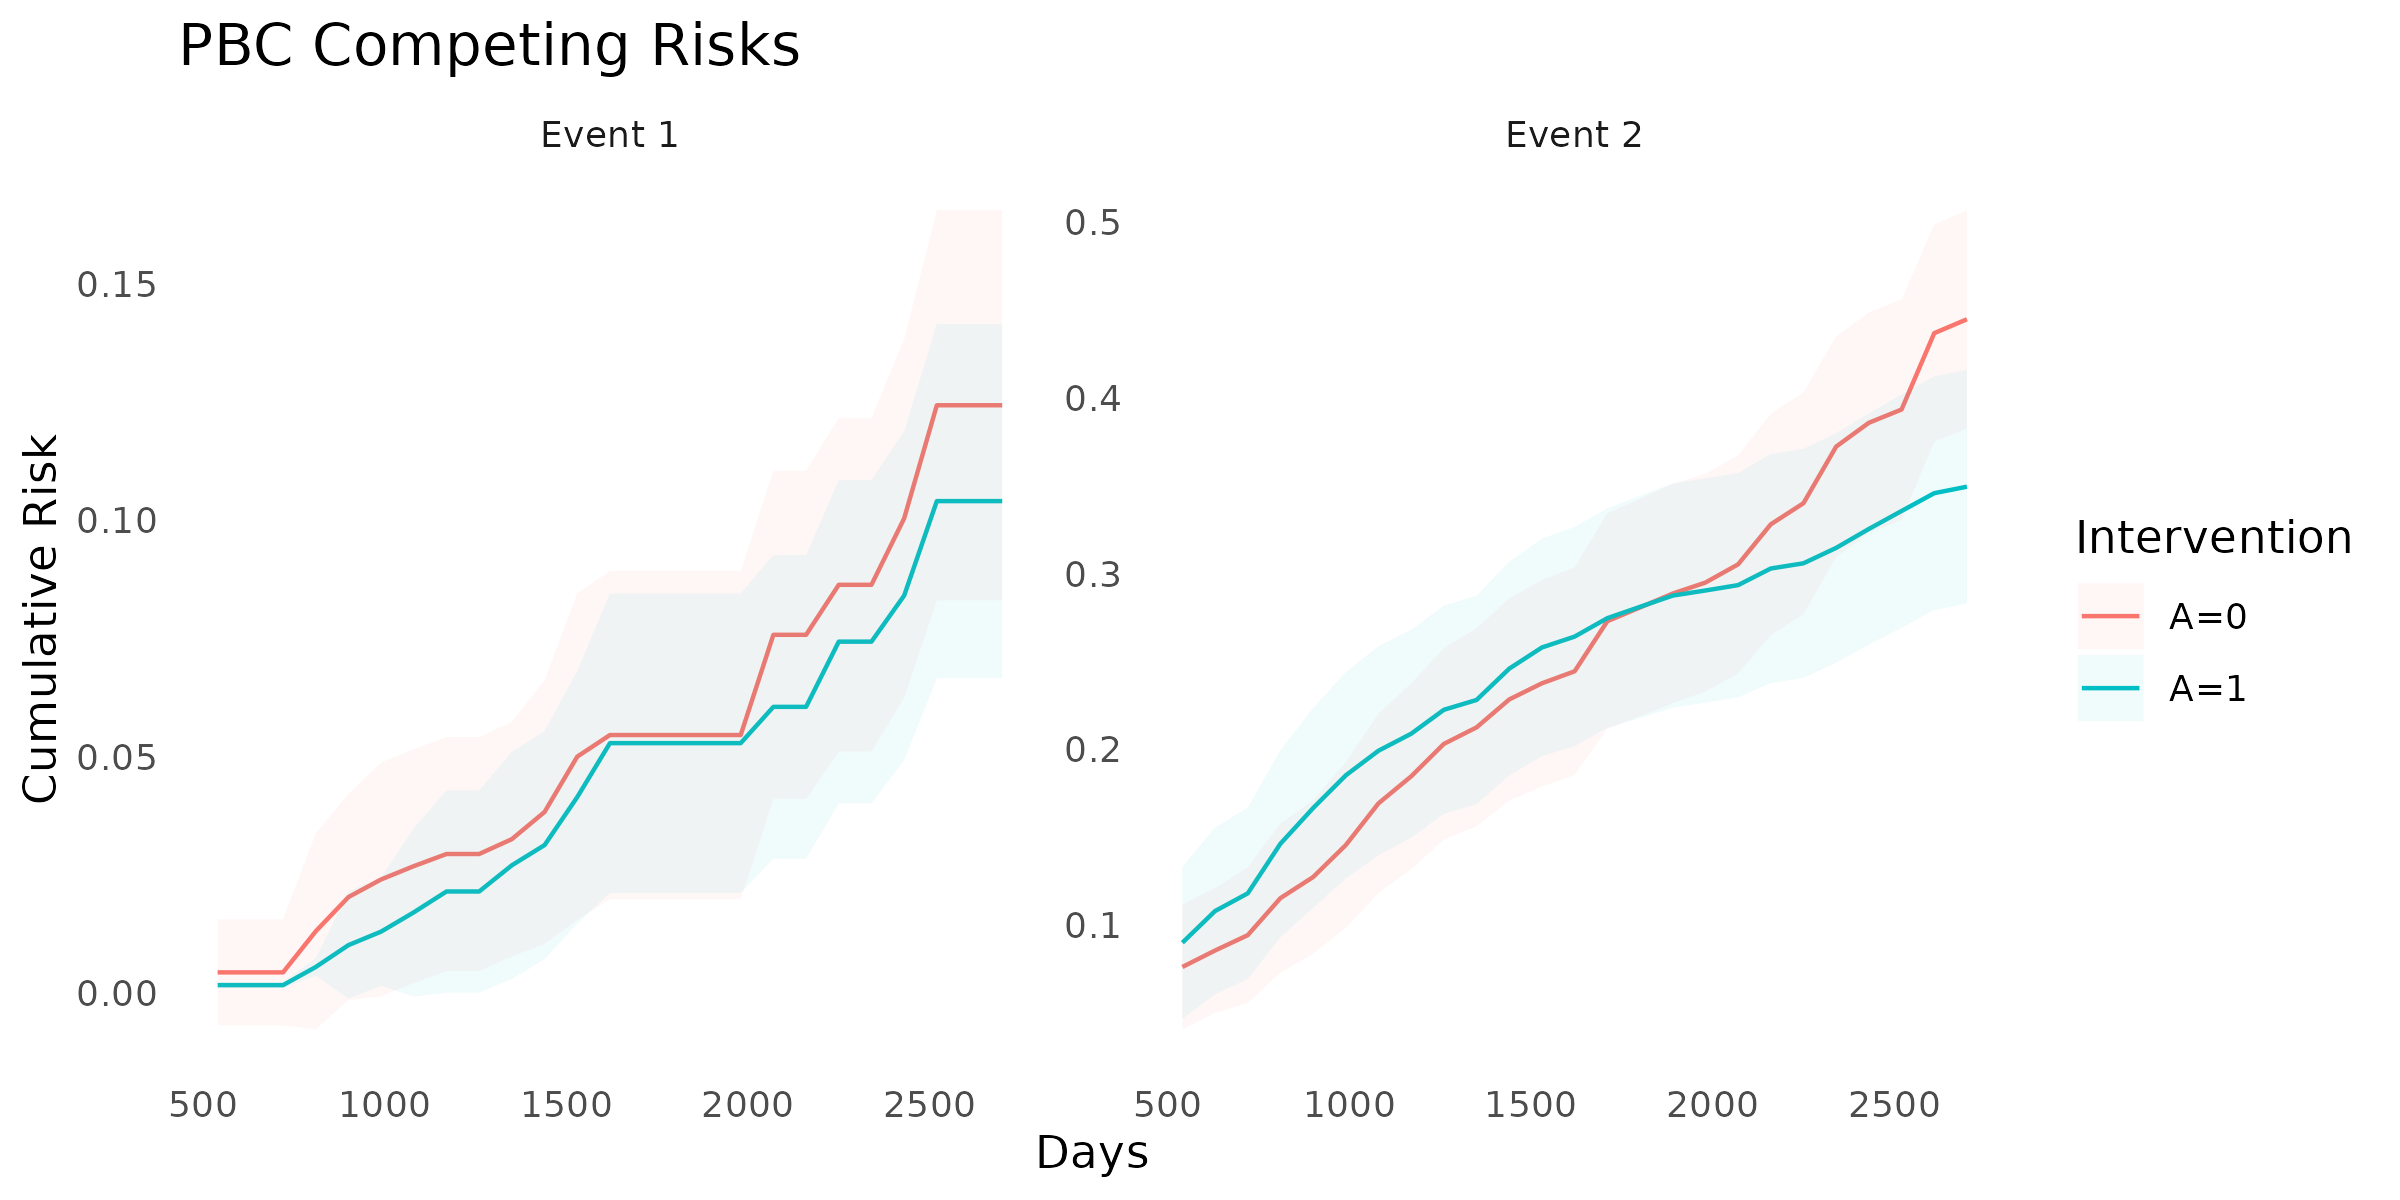
\includegraphics[width=\linewidth]{fig/concrete-pbc.png}
\end{figure}

Here, by comparing the treated and control cumulative incidence curves we can more clearly see the effect of treatment on incidence of both transplant and death, and especially how the treatment effect on risk of death varies over time. 

\section{Diagnostics and Debugging}
\label{sec:org023a4af}
\subsection{ConcreteArgs}
\label{sec:org3aaa14e}
The print method for ConcreteArgs objects displays summary information about 1) the observed data, 2) the target estimand (i.e. target event(s), target time(s) and intervention(s)), 3) specifications for initial nuisance parameter estimation, and 4) specification for the TMLE update. 

\lstset{language=r,label= ,caption= ,captionpos=b,numbers=none,otherkeywords={}, deletekeywords={}}
\begin{lstlisting}
print(ConcreteArgs, Verbose = FALSE)
\end{lstlisting}

\begin{figure}[H]
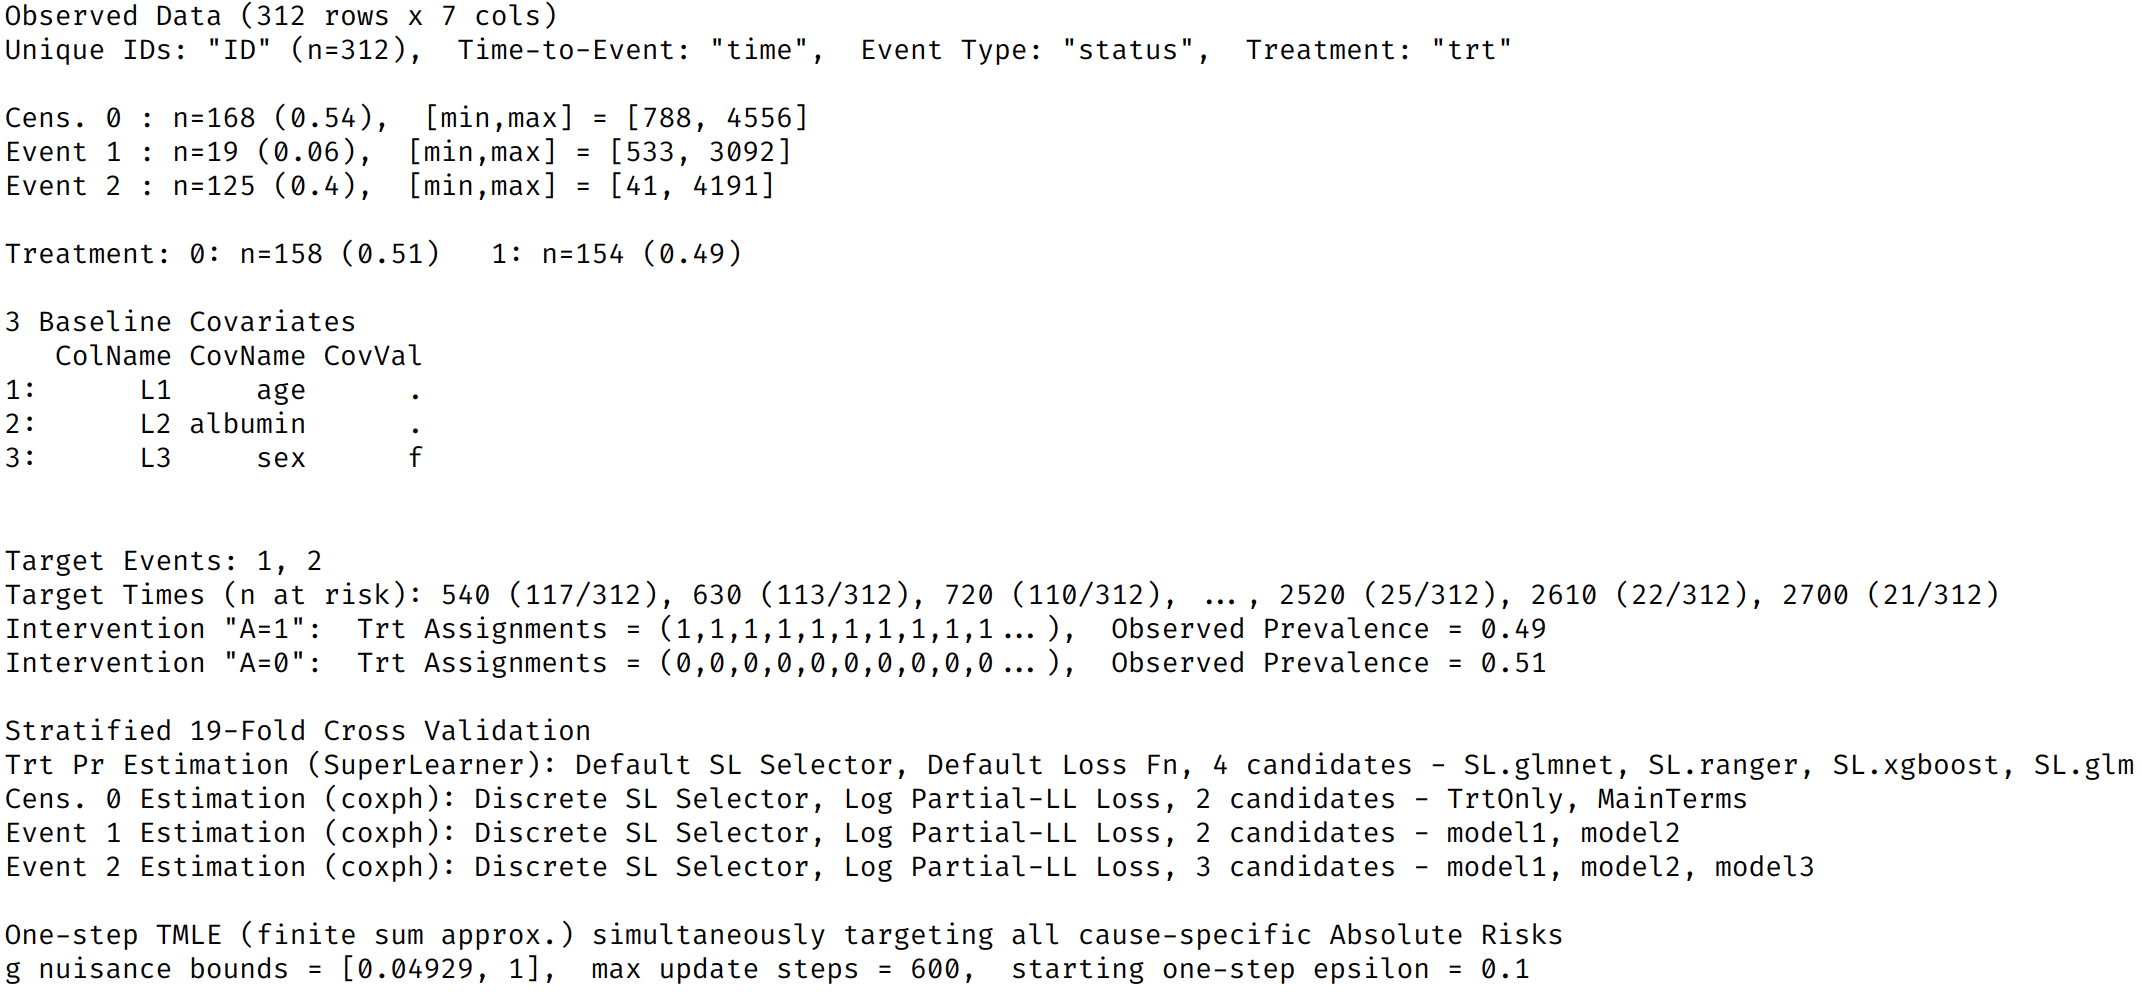
\includegraphics[width=\linewidth]{fig/ConcreteArgs.png}
\end{figure}

\subsection{ConcreteEst}
\label{sec:orge61cf9e}
The print method for ConcreteEst objects displays information about whether TMLE adequately converged, truncation of intervention-related nuisance parameter estimates, and the initial estimation of nuisance parameters.

\lstset{language=r,label= ,caption= ,captionpos=b,numbers=none,otherkeywords={}, deletekeywords={}}
\begin{lstlisting}
print(ConcreteEst)
\end{lstlisting}

\begin{figure}[H]
\center
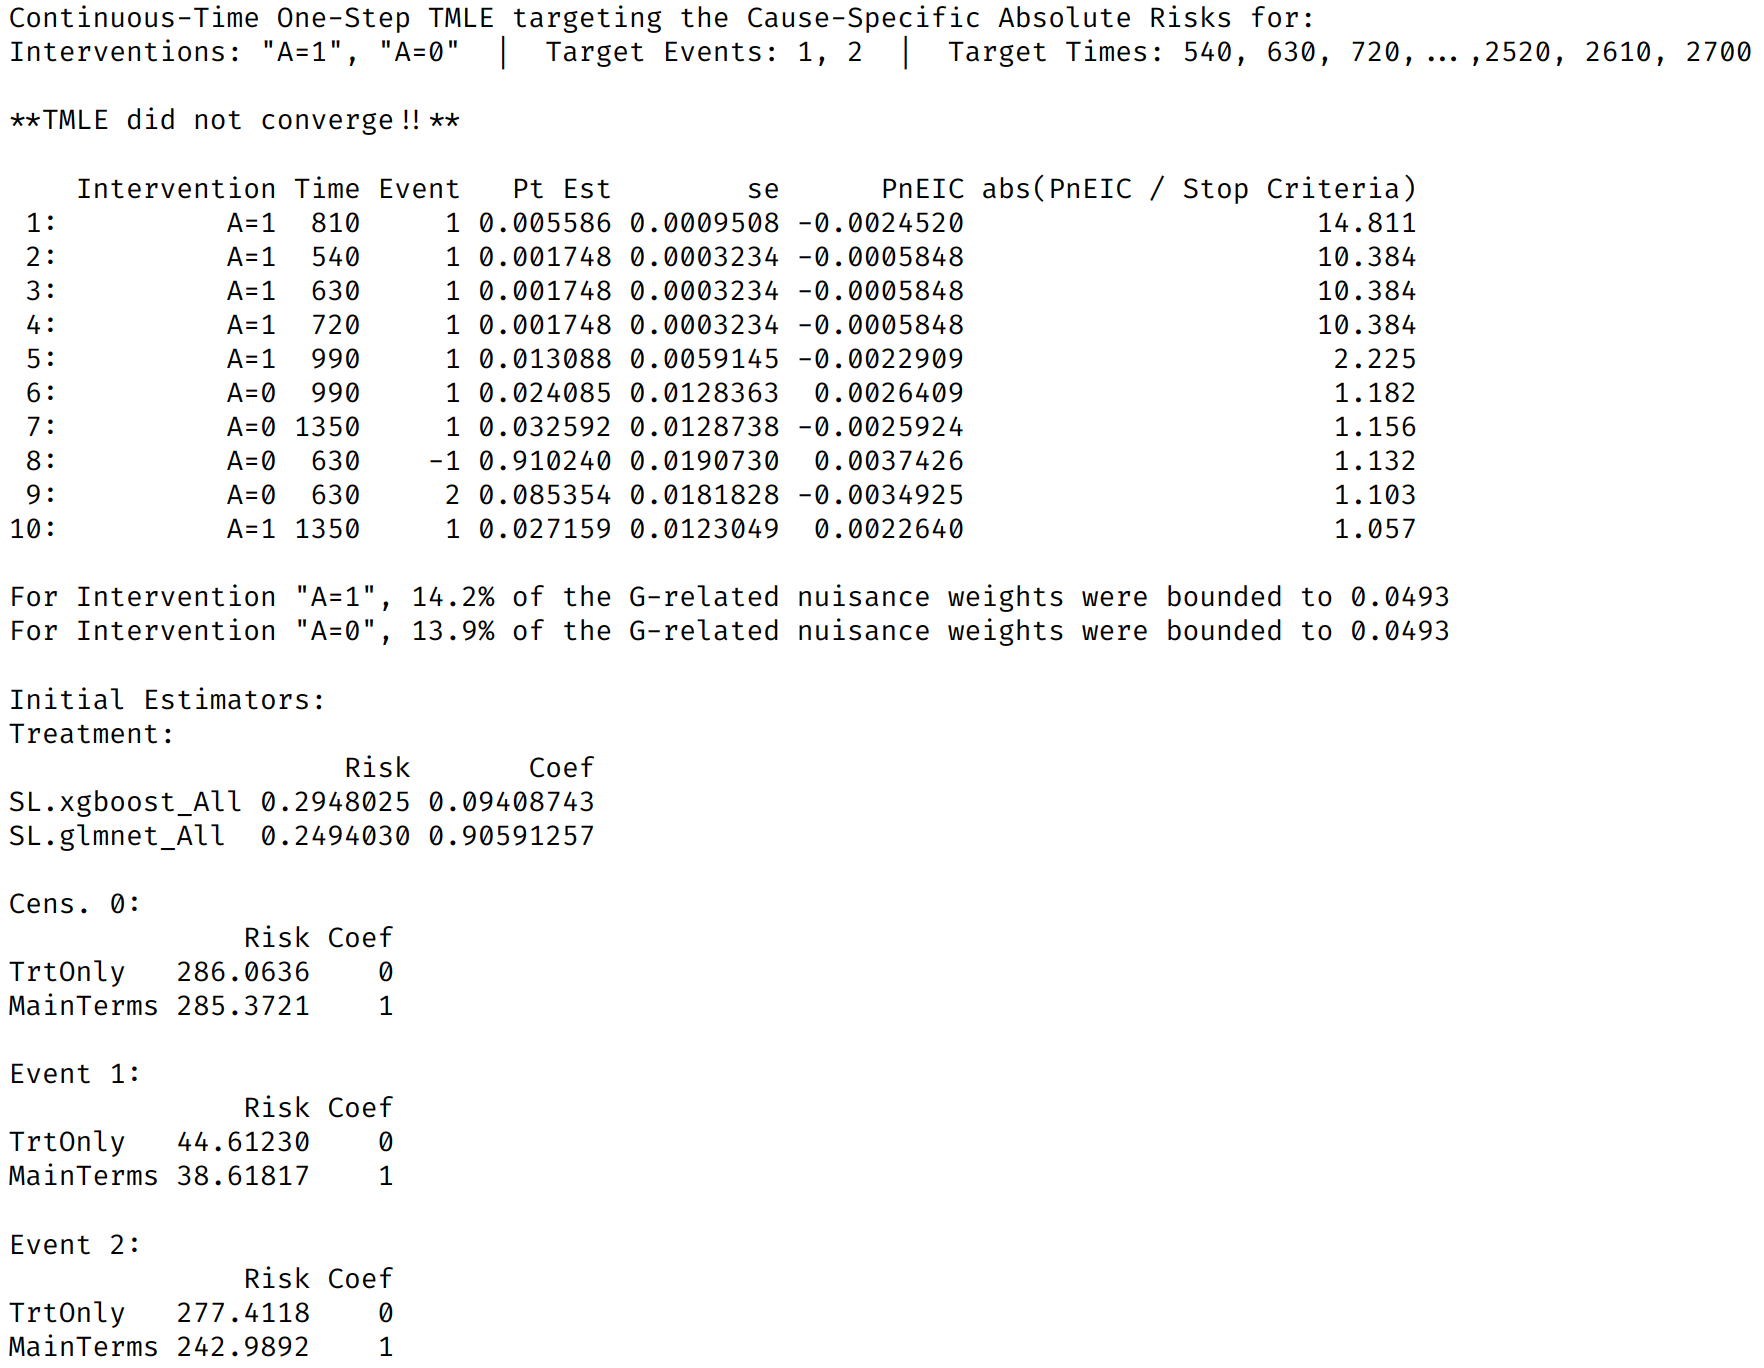
\includegraphics[width=\linewidth]{fig/ConcreteEst.png}
\end{figure}

If TMLE has not converged, the mean EICs that have not attained the desired cutoff will be displayed in a table. As can be seen above, when few events have yet occurred by some targeted times even small PnEICs may not meet the convergence criteria and precisely estimating event incidence may simply not be possible given the observed data. Otherwise, TMLE convergence may be attained by increasing the maximum number of TMLE iterations.

The print method for ConcreteEst objects shows the amount of g-related nuisance parameter truncation for each intervention and for more details the plot method for ConcreteEst objects plots the distribution of estimated propensity scores for each intervention. Propensity scores close to 0 indicate the possibility of posivity violations and may warrant re-examining the target time(s), interventions, and covariate adjustment sets.

\begin{figure}[H]
\center
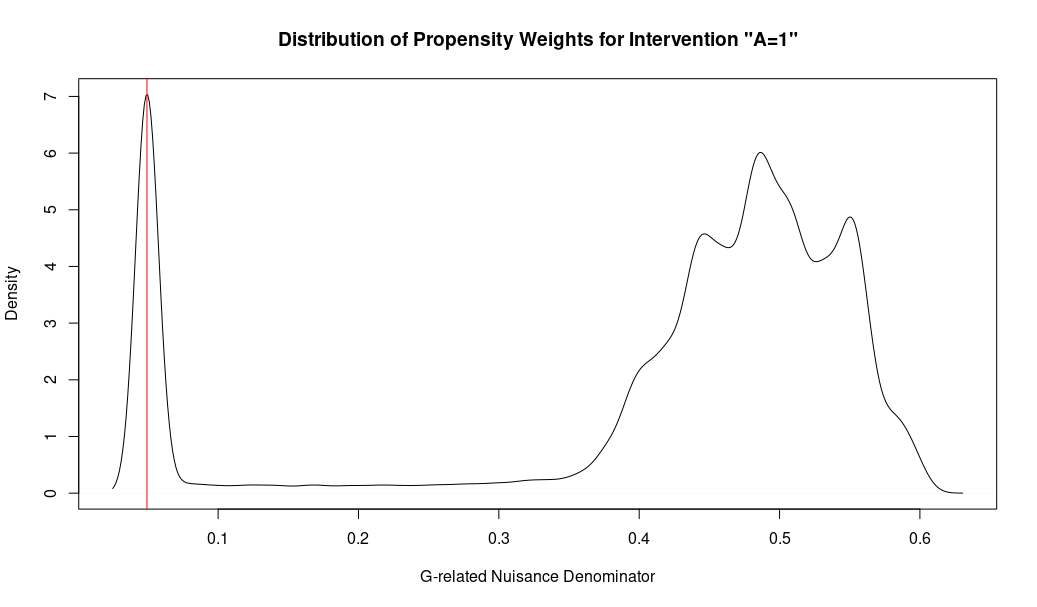
\includegraphics[width=\linewidth]{fig/A1-propscores.png}
\end{figure}

\subsection{Nuisance Weight Truncation Simulation}
\label{sec:org48001b2}


\section{Appendix: Nice to have Concepts}
\label{sec:org0ff7c78}

\subsection{Identification}
\label{identification}
In order to identify causal estimands such as absolute risk ratios and differences with functions of the observed data, some untestable structural assumptions must hold - namely the assumptions of consistency, positivity, randomization, and coarsening at random on the conditional density of the censoring mechanism. 


\begin{enumerate}
\item The consistency assumption states that the observed outcome given a certain treatment decision is equal to the corresponding counterfactual outcome
\end{enumerate}
\[ T^d_j = T_j \text{ on the event that A = d(L)} \]

\begin{enumerate}
\item The positivity assumption states that the desired treatment regimes occur with non-zero probability in all observed covariate strata, and that remaining uncensored occurs with non-zero probability in all observed covariate strata at all times of interest \(t\).
\end{enumerate}
\[ P_0\left( A = d(L) \mid \L \right) > 0 \;,\, a.e. \]
\[ P(C \geq t \mid a, \L) \;,\, a.e. \]

\begin{enumerate}
\item The randomization assumption states that there is no unmeasured confounding between treatment and counterfactual outcomes
\end{enumerate}
\[ A \indep (T^d_1, T^d_2) \mid \L \]

\begin{enumerate}
\item Coarsening at random on censoring
\end{enumerate}
\[ C \indep (T^d_1, T^d_2) \mid T > C, A, \L \]

Given coarsening at random, the observed data distribution factorizes 
\begin{align*}
p_0(O) = p_{0}(\L)\, \g_0(A \mid \L)\, \lambda_{0,c}&(\T \AX)^{\1(\Delta = 0)} S_{0, c}(\T\text{-} \AX)\\
&\prod_{j=1}^{J} S_{0}(\T\text{-} \AX) \, \lambda_{0,j}(\T \AX)^{\1(\Delta = j)}
\end{align*}
where \(\lambda_{0,c}(t \AX)\) is the true cause-specific hazard of the censoring process and \(\lambda_{0,j}(t \AX)\) is the true cause-specific hazard of the \(j^{th}\) event process. Additionally
\begin{align*}
    S_{0,c}(t \ax) &= \exp\left(-\int_{0}^{t} \lambda_{0,c}(s \ax) \,ds\right)
\intertext{while in a pure competing risks setting}
    S_0(t \ax) &= \exp\left(-\int_{0}^{t} \sum_{j=1}^{J} \lambda_{0,j}(s \ax) \,ds\right)
\intertext{and} 
    F_{0,j}(t \ax) &= \int_{0}^{t} S(s\text{-} \ax) \lambda_{0,j}(s \ax)\,ds\\
    &= \int_{0}^{t} \exp\bigg(-\int_{0}^{s} \sum_{j=1}^{J} \lambda_{0,j}(u \ax)\,du\bigg) \lambda_{0,j}(s \ax)\,ds.
\end{align*}

Under the above identification assumptions, the post-intervention distribution of \(O\) under intervention \(A=d(a, \l)\) in the world of no-censoring, i.e the distribution of \((\L,\, T^d_j,\, \Delta^d_j :\, j = 1, \dots, J)\), can be represented by the so-called G-computation formula. Let’s denote this post-intervention probability distribution with \(P_{d}\) and the corresponding post-intervention random variable with \(O_d\). The probability density of \(O_d\) follows from replacing \(\g_0(A \mid \L)\) with the density that results from setting \(A = d(a, l)\), \(\g_d(d(A, \l) \mid \L)\), and replacing the conditional probability of being censored at time \(t\) by no censoring with probability \(1\). In notation, \(P(O_d = o)\) is given by
\begin{align*}
p_{d}(o) = p_{0}(\l) \, &\g_d(d(a, \l) \mid \l) \, \1(\delta \neq 0)\\
&\prod_{j=1}^{J} \left[S_{0}(\t\text{-} \mid A = d(a, \l),\, \l) \, \lambda_{0,j}(\t \mid A = d(a, \l), \l)^{\1(\delta = j)} \right]
\end{align*}
Recalling the censoring and cause-specific conditional hazards defined above in terms of observed data, we should note that given the identifiability assumptions they now identify their counterfactual counterparts, i.e. 
\[\lambda_{c}(t \mid W,\, A) = \lim_{h \to 0}P(C < t + h \mid C \geq t,\, W,\, A)\]
\[\lambda_{j}(t \mid W,\, A)= \lim_{h \to 0}P(T < t+h, J=j \mid T \geq t, W, A)\]
Note that the cause-specific event hazards are not conditional on censoring once identifiability assumptions are met.

Since the density \(P(O_d=o)\) implies any probability event about \(O_d\), this g-computation formula for \(P(O_d=o)\) also implies g-computation formulas for causal quantities such as event-free survival and cause-\(k\) absolute risk under intervention \(d\). 

\newpage
\bibliography{main.bib}
\end{document}